% main text for the telluric section in keck.tex
%%%%%%%%%%%%%%%%%%%%%%%%%%%%%%%%%%%%%%%%%%%%%%%%%%%%%%%%%%%%%%%%%%%%%%%%%%%%
%%%%%%%%%%%%%%%%%%%%%%%%%%%%%%%%%%%%%%%%%%%%%%%%%%%%%%%%%%%%%%%%%%%%%%%%%%%%
\subsection{Introduction}\label{keck:telluric:intro}

The first exoplanets around main-sequence stars were discovered by the
radial velocity (RV) method, where precise Doppler spectroscopy
measures the wavelength shift of the host stars induced by the
gravitational pull of the planets \citep{1988ApJ...331..902C,
  1989Natur.339...38L, 1993ApJ...413..339H, 1995Natur.378..355M,
  1996ApJ...464L.153B}. Since then, the RV method has discovered
hundreds of planetary systems (see exoplanets.org; \citealt{eod2014})
and contributed to numerous confirmation and characterization of
exoplanets discovered by the transit method (e.g., for
\kepler\ follow-up observations; \citealt{Marcy2014}).

The current best RV precision is around 1~m/s \citep{eprv2015},
attainable via two wavelength calibration methods in the optical band:
ThAr lamp emission line calibration (e.g., ELODIE and HARPS;
\citealt{elodie, harps-s}; $\sim$400-690~nm) and iodine cell
absorption line calibration (e.g., Keck/HIRES and Magellan/PFS;
\citealt{butler1996, 2010SPIE.7735E..53C}; $\sim$500-620~nm). The
major obstacles for achieving a higher RV precision are: stellar
activity induced RV signals, instrumental effects, telluric
contamination, and limitation in data analysis \citep{eprv2015}.

Traditionally, telluric contamination is not considered as problematic
for precise RV in the optical. It is certainly a sever source of
spectral contamination and a bottleneck for achieving higher RV
precision in the near infra-red (NIR) region (e.g.,
\citealt{2010ApJ...713..410B}), where a large number of deep water and
methane lines reside. However, there is only a small wavelength
range in the optical that has deep telluric lines, and typically such
regions are simply thrown out for the purpose of precise RV analysis,
either by giving them zero weights in the cross correlation masks (for
ThAr calibrated spectra, e.g., \citealt{2002A&A...388..632P}) or
flagging them as bad pixels (for iodine calibrated spectra, e.g., for
Keck/HIRES).

Recently, the works by \cite{artigau2014} and \cite{cunha2014} have
characterized and mitigated the effects of telluric contamination in
the precise RV data taken by the ThAr-calibrated HARPS-S.
\cite{cunha2014} focuses on the issues with ``micro-telluric" lines
(shallow telluric absorption lines with $<1$-3\% depths), which are
recognized for the first time. \cite{cunha2014} fit and then divide
out the telluric lines in the observed spectra using synthetic
telluric spectra generated by the LBLRTM package (Line-By-Line
Radiative Transfer Model, \citealt{lblrtm}; with line lists from
HIgh-resolution TRANsmission molecular absorption database, or HITRAN,
\citealt{hitran2013}) and also TAPAS \citep{tapas}, which is a more
user-friendly but less flexible package wrapper using LBLRTM. They
concluded that the micro-tellurics have an impact (defined as RMS of
difference between RVs before and after micro-telluric removal) of
$\sim$10-20 cm/s for G stars observed with low to moderate air masses,
but the impact can be substantial in some cases to up to $\sim$0.5-1
m/s.

\cite{artigau2014} uses principal component analysis (PCA) to
empirically correct for telluric lines in HARPS-S data (both
micro-tellurics and the deep lines in the $\sim$630~nm region), and
combined PCA with rejection masking, they reduced the RV RMS by
$\sim$20~cm/s (and more significantly for the $\sim$630~nm
region). More recently, \cite{2016AAS...22713719S} characterized the
effects of telluric contamination and effectiveness of some typical
remedies (masking and modeling) for emission line-calibarated spectra
for the optical, broad optical (300-900~nm), and NIR. Their conclusion
for the optical region is similar to the results in \cite{artigau2014}
and \cite{cunha2014}.

This paper characterizes and corrects for the adverse effects of
telluric contamination under the context of iodine-calibrated precise
RV, especially for the micro-telluric lines. ZZZ We first describe our
methodology for characterizing the effects of tellurics in
Section~\ref{keck:telluric:method}, then... ZZZ


%----------------------------------------------------------------
% Plot showing micro-telluric lines
% made by ~/Exo../Keck../plots_general/spec_plot.pro
\begin{figure}
\includegraphics[scale=0.5]{telluric/tellurics_all.eps} 
\caption{Telluric lines in the iodine region are mostly shallow water
lines, with some moderately deep water lines near 5900\AA\ and very
deep oxygen lines near 6300\AA. The insert plot is showing the
pervasiveness of micro-telluric lines, i.e.~$\leq$1--3\% in depths.
\label{telluric:fig:telluric}}
\end{figure}
%----------------------------------------------------------------



%%%%%%%%%%%%%%%%%%%%%%%%%%%%%%%%%%%%%%%%%%%%%%%%%%%%%%%%%%%%%%%%%%%%%%%%%%%%
%%%%%%%%%%%%%%%%%%%%%%%%%%%%%%%%%%%%%%%%%%%%%%%%%%%%%%%%%%%%%%%%%%%%%%%%%%%%
\subsection{Impacts of Micro-tellurics on RV Precision}\label{keck:telluric:method}

We performed end-to-end simulation of Keck data and analysis process
to access the impacts of micro-tellurics on RV precision. We use Keck
to demonstrate this because Keck has the highest precision. We chose
sig Dra and tau Ceti as our stars because they are RV standards which
have been observed hundreds of times with Keck/HIRES, and are also
favorite RV standards at other precise RV facilities. I really want to
add an M dwarf standard here as well!


%%%%%%%%%%%%%%%%%%%%%%%%%%%%%%%%%%%%%
\subsubsection{Methodology}

We simulated Keck observations on sig Dra and tau Ceti by using
synthetic stellar spectra of their respective spectral types (?) using
SME (ZZZ cite Valenti and Fischer). We simulated one spectrum for each
actual observed spectrum taken at Keck through the CPS programs. The
synthetic stellar spectra is multiplied with the iodine atlas to
create the standard iodine$+$ star RV observations. The multiplied
spectrum is then multiplied with the blaze function and convolved with
the observed spectral PSF, both derived from real observations for
each night. Poisson noise is added.

We then forward model the simulated spectra to extract RVs using the
CPS Keck code (ZZZ cite Johnson and Howard). We used the synthetic
stellar spectrum as the input stellar template. In reality, stellar
templates are derived from observed stellar spectra via deconvolution,
which would introduce additional errors. Using the same synthetic
stellar spectrum would eliminate such errors and isolate the problem
to telluric lines only.

We ran two sets of simulations: control and contaminated. In the
control, we only had stellar spectrum and iodine spectrum. In the
contaminated, we added in simulated telluric lines in the simulated
observed spectrum. The telluric lines were generated using TERRASPEC
(ZZZ cite Bender). We adopted the typical Mauna Kea atmospheric
condition (temperature and pressure profiles) and typical oxygen
column density (which in realiaty flucturate very little anyway). For
simplicity, we assumed the same water column density for every
observation, which is pwv$=1$mm, a little bit humid than a typical
Mauna Kea night (true? I think this is actually pretty typical). The
pair of simulated control and contaminated spectra have the same added
Poisson noise, and therefore any RV differences derived from these two
sets of simulation would reveal the net effect of telluric
contamination.


%%%%%%%%%%%%%%%%%%%%%%%%%%%%%%%%%%%%%
\subsubsection{Results}

%----------------------------------------------------------------
% Telluric effect, no photon noise
% plot made by ~/Exo.../Keck.../simulate.../msplot.pro
\begin{figure}
\subfloat{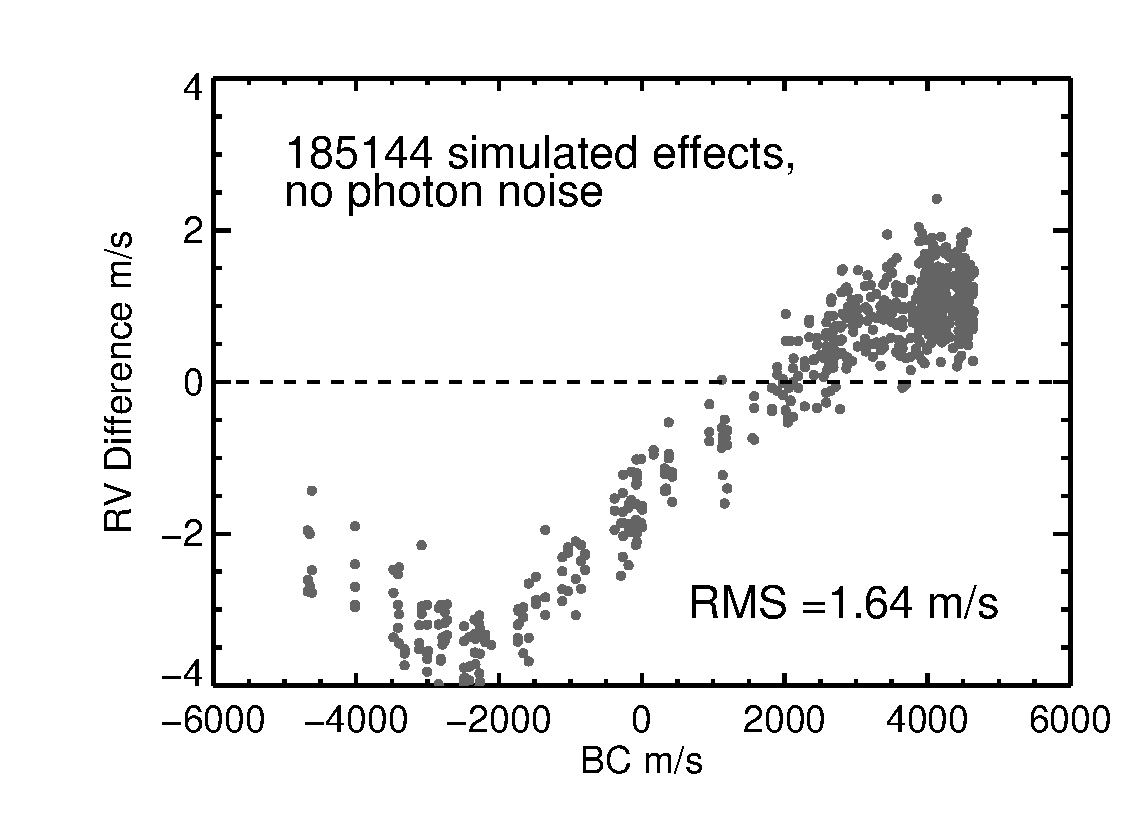
\includegraphics[scale=0.38]{telluric/185144-rv-bc-rja01-rjb01.eps}}\
\subfloat{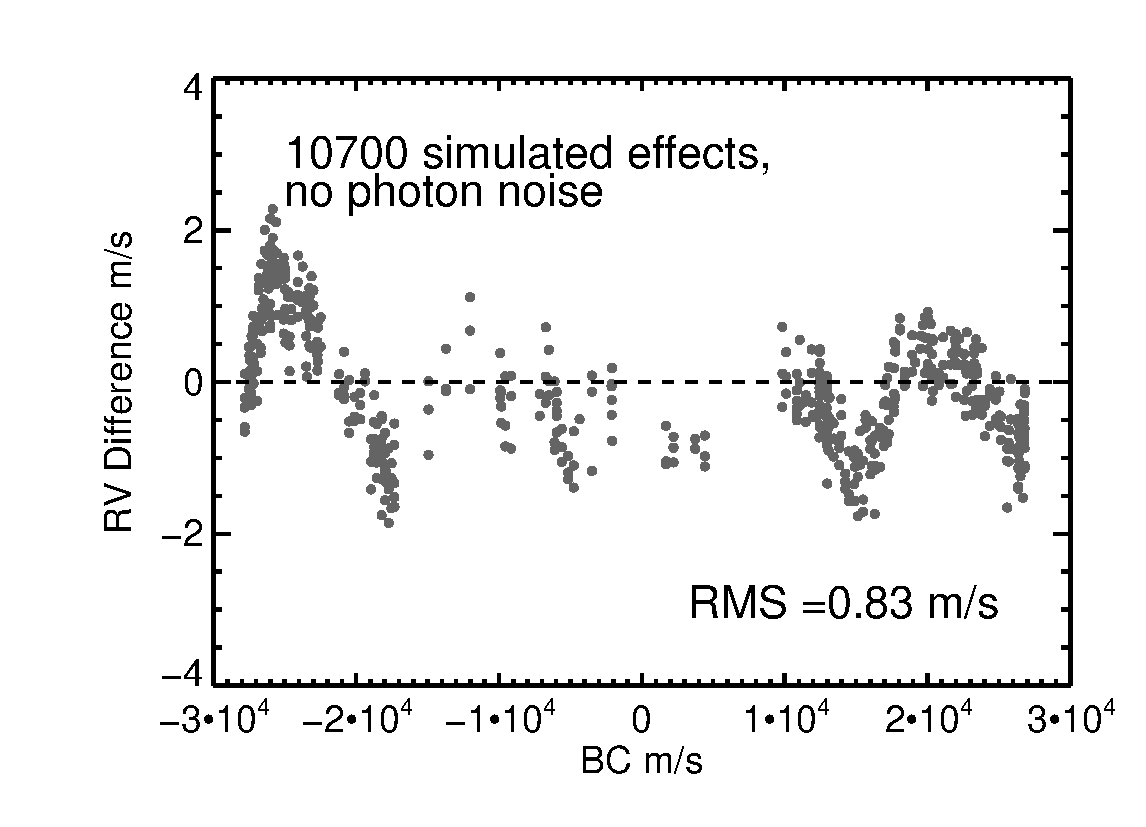
\includegraphics[scale=0.38]{telluric/10700-rv-bc-rja01-rjb01.eps}}\
\subfloat{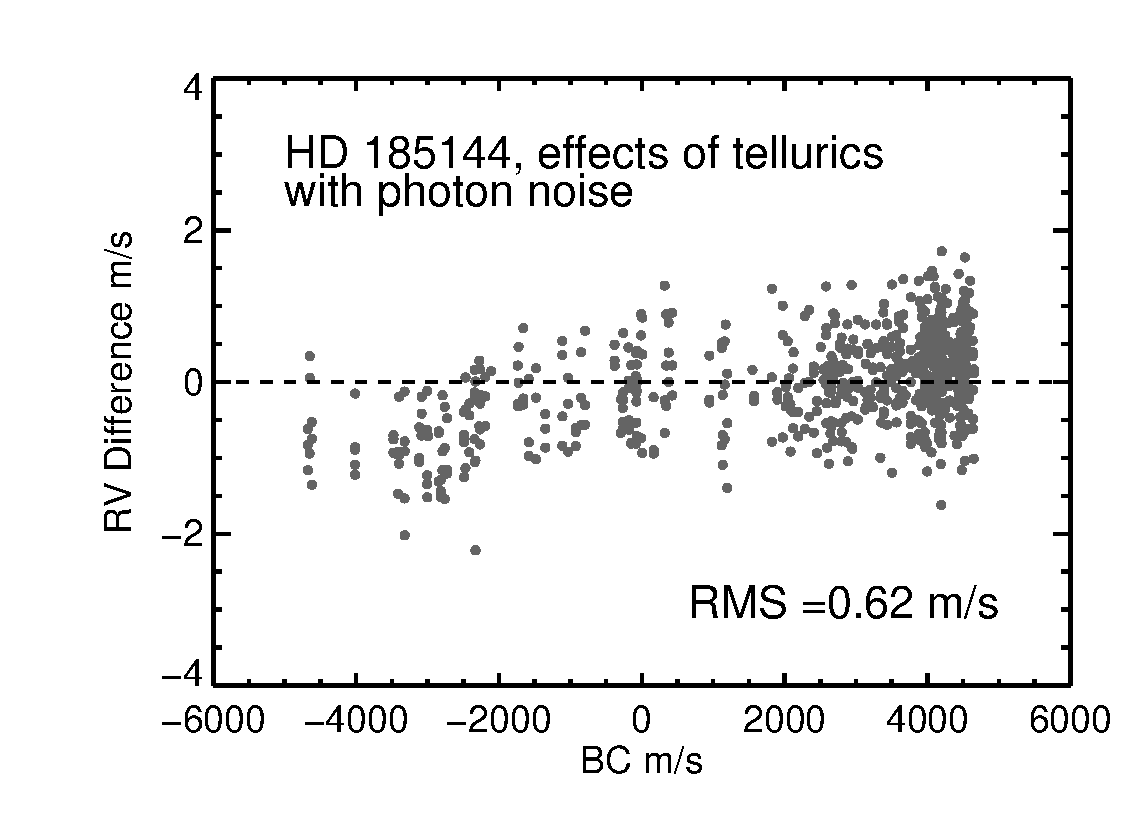
\includegraphics[scale=0.38]{telluric/185144-rv-bc-rjc01-rjd01.eps}}\
\subfloat{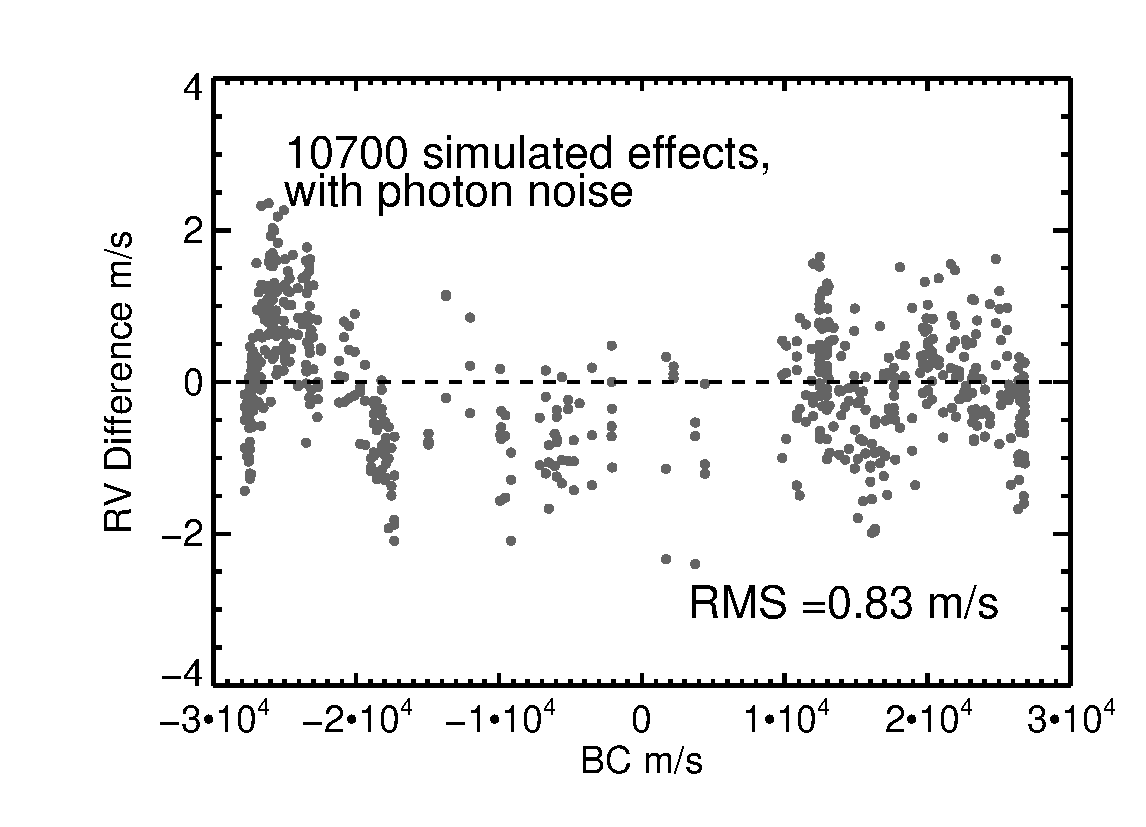
\includegraphics[scale=0.38]{telluric/10700-rv-bc-rjc01-rjd01.eps}}\
\subfloat{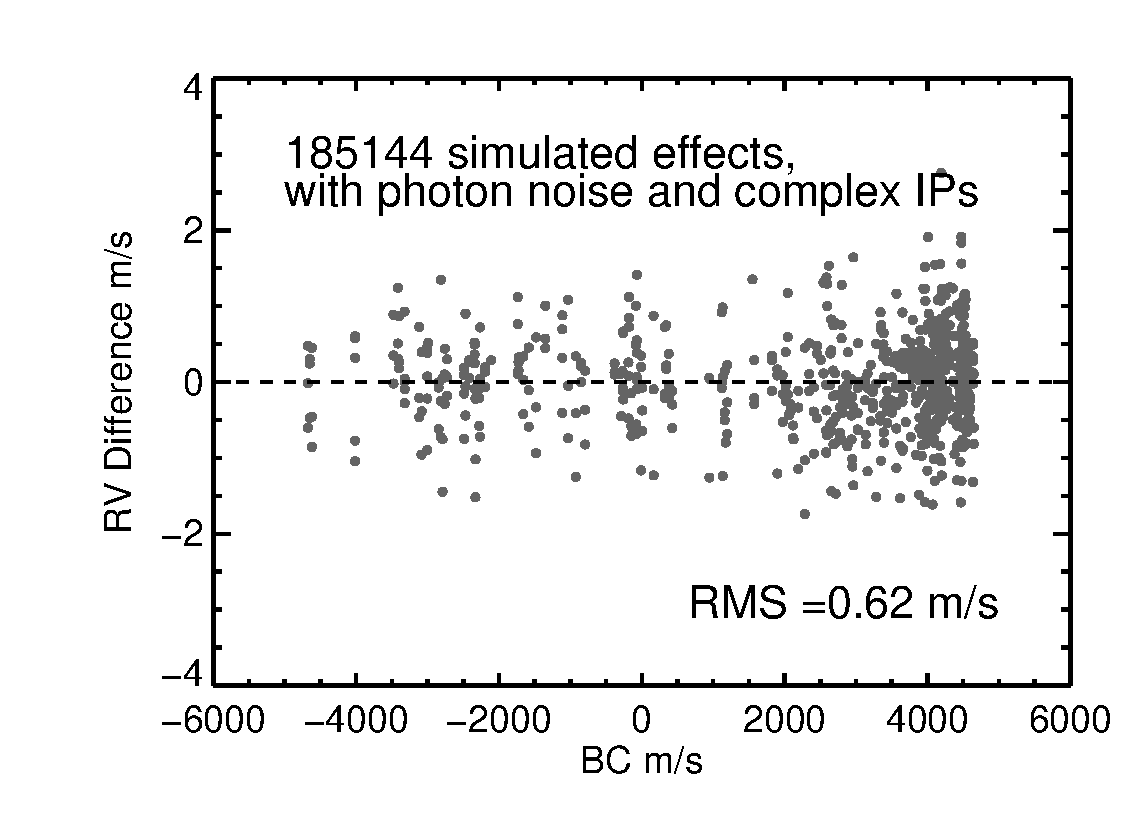
\includegraphics[scale=0.38]{telluric/185144-rv-bc-test0-test1.eps}}\
\subfloat{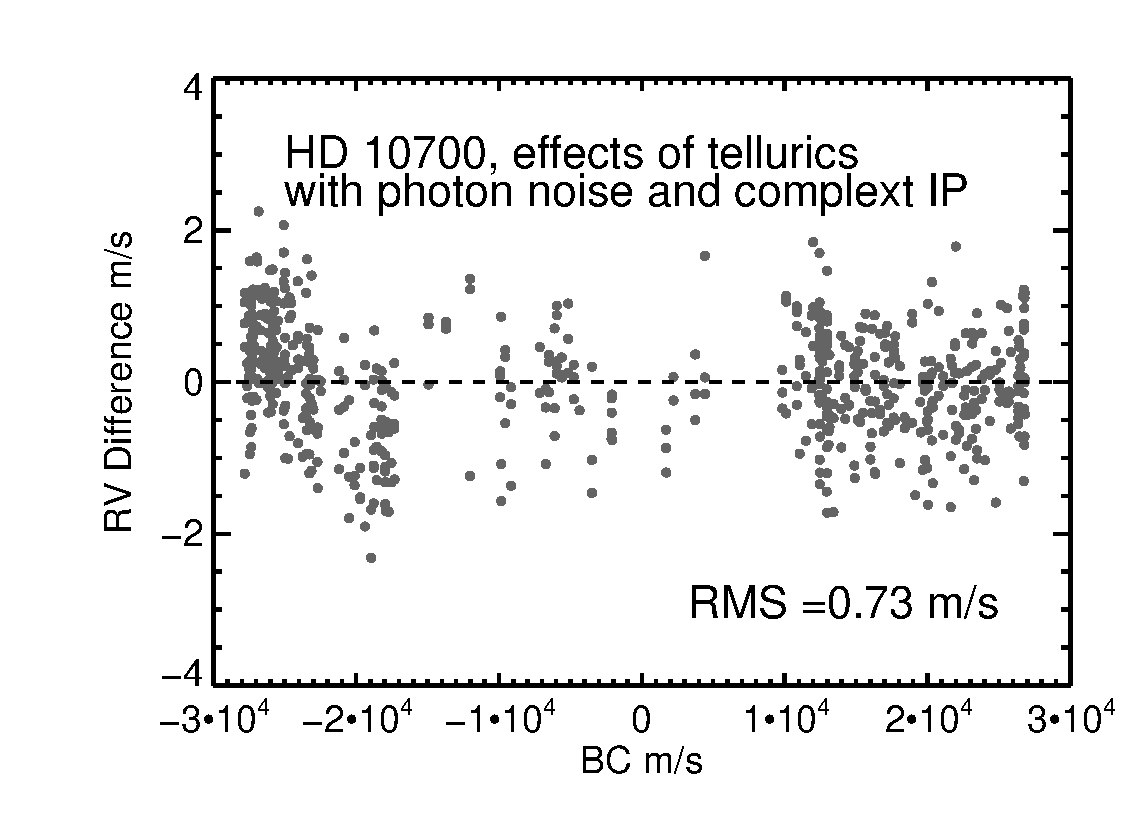
\includegraphics[scale=0.38]{telluric/10700-rv-bc-test0-test1.eps}}
\caption{Effects of telluric lines manifested as correlation between
  RV and BC. Each point represents the difference in RV estimates for
  a pair of simulated spectra: one without telluric absorption, and
  one with telluric absorption on top of the stellar and iodine
  spectra. {\bf Top 2 panels:} To isolate the effects of telluric
  lines, the simulated spectra used for this plot do not have Poisson
  noise added, and they have simple one-component Gaussian IPs which
  have fixed width and thus the IP parameters are all fixed to the
  true values in the RV extraction. {\bf Middle 2 panels:} same as the
  top panels, but for simulated spectra with Poisson noise (same noise
  for the telluric and non-telluric spectrum pairs; and still the same
  simple IPs). {\bf Bottom 2 panels:} same as above, but for simulated
  spectra with Poisson noise and complex IPs that are similar to the
  ones in actual observations. IP parameters are not fixed in this
  case, so the code is fitting 12 additional parameters for the IP on
  top of the 3 for wavelength solution and Doppler shift (see
  Chapter~\ref{chap:doppler} for more details on the code).
\label{telluric:fig:sim}}
\end{figure}
%----------------------------------------------------------------


Micro-tellurics in the iodine region introduces RMS$=0.6$ m/s scatter
for GK stars (RV systematic error added in quadrature). Leaving
untreated, this would define the precision floor.

Additionally, it manifests as spurious signal at periods of a sidereal
year and harmonics, with an amplitude of 20 cm/s. This would affect
our ability to detect super-Earth in the habitable zone of GK stars
(Earth's signal is 8 cm/s). We have seen such spurious signal in Keck
data on many stars, and telluric contamination is one of the
contributing factors (see discussion for other factors).

For M stars... (probably worse)


%%%%%%%%%%%%%%%%%%%%%%%%%%%%%%%%%%%%%%%%%%%%%%%%%%%%%%%%%%%%%%%%%%%%%%%%%%%%
%%%%%%%%%%%%%%%%%%%%%%%%%%%%%%%%%%%%%%%%%%%%%%%%%%%%%%%%%%%%%%%%%%%%%%%%%%%%
\subsection{Remedies and Effectiveness}

There are several ways to remedy the adverse effects of telluric lines
on RV precision and accuracy: masking, modeling, or a combination of both.

% why simple masking would not work for high precision/accuracy
First, we can simply mask out the telluric lines in the observation
(and also in the deconvolved stellar reference spectrum). For each
observation, we can locate the pixels contaminated by telluric lines,
and flag them as bad pixels so that the fitter would ignore them. This
is done ``dynamically'' in the fitting process, in the sense that, for
each iteration in the least-$\chi^2$ minimization process, the
contaminated pixels are located according to the current wavelength
solution parameters in this fitting iteration. The wavelength solution
changes from iteration to iteration, and thus the masked pixels can
change too. One can easily see that this introduces some
complications. First of all, the degrees of freedom might change
during the fitting, because some telluric lines may shift in and out
of this spectral chunk as the wavelength solution changes. As a result, a
dynamic mask complicates the $\chi^2$ surface and would make the
fitter harder to converge or may create more loci for the fitter to
get stuck in, causing additional errors. Furthermore, masking is throwing
away iodine and stellar content embedded in these pixels too. Finally, to
``mask'' the telluric lines out, one needs to pick a flux threshold,
say, masking all telluric absorption deeper than 0.5\% level. This
number is hard to choose, because masking too much would throw away
too many iodine and stellar pixels, but masking too little would mean
leaving shallow telluric lines and line wings that can still cause
biased RV estimates. We have determined that n\% is the best...

double masking: probably a terrible idea. Throwing away the
pixels will make the fitter harder to converge, and introduce
additional errors on the scales larger than the effects of telluric
lines themselves. Additionally, it is hard to choose a flux cut-off
level. Throwing away too much would mean unstable solution and lower
RV precision, but masking too little would mean insufficient removal
of tellurics.

% modeling is the way to go
The other way is to incorporate telluric lines as part of the iodine
RV forward modeling process, where water column density can either be
from a priori knowledge or an additional free parameter. While
modeling is shown to be a better approach to the problem (see the
following subsection), it is not free of troubles: telluric lines can
be notoriously hard to model to high precision (below 1\% RMS
residual). There are several reasons for this: lab measurements of a
large number of water lines are inaccurate, in terms of line depths,
line positions, and line shapes; and these line properties can also
change due to change or a lack of knowledge of the atmospheric
conditions, such as wind, high line-of-sight variations (e.g., water
vapor), and mixing uncertainties. For a summary of the state of the
problem and recommendations of paths forward recommended by the RV
community, see Section~4.6 in \cite{eprv2015}. However, the goal here
is not to model or ``remove'' the telluric lines perfectly, but to
mitigate their impact on RV precision and accuracy as much as
possible, which is discussed in detail in the following subsection.

% but combination of the two could be better 
Additionally, the weighing procedure or ``vanking'' in the CPS Doppler
code is essentially performing some ``masking'' on the chunks that are
badly contaminated by tellurics, such as the ones near 6300\AA\ with
deep oxygen lines and little stellar or iodine content. Such oxygen
chunks are normally thrown out completely, and other contaminated
chunks which suffer from low precision will receive lower weights and
thus cast a lower impact on the final precision and
accuracy. Therefore, with this ``masking'' mechanism already in place,
further incorporating in forward modeling of telluric line is the
optimal solution to the problem. We will discuss the complications
with real observations in the second subsection.


\subsubsection{How precisely does one need to model the tellurics?}

realistically
speaking, below a certain threshold set by science requirement. As
discussed in the following subsection, it does not require perfect
modeling (e.g., below 1\% flux residual) of tellurics to control the
introduced RV RMS to below 10~cm/s in the RV error budget for the
iodine-calibrated RVs or probably RVs in the (short) optical region in
general \citep{cunha2014, artigau2014}. For redder bands, it is
unclear at the moment what the requirement would be, although some
theoretical calculation by \cite{2016AAS...22713719S} suggests that
modeling to 1\% may not be sufficient for reaching below 1~m/s in the
near infrared.

%----------------------------------------------------------------
% NEID Plot showing how much you need to model tellurics
\begin{figure}
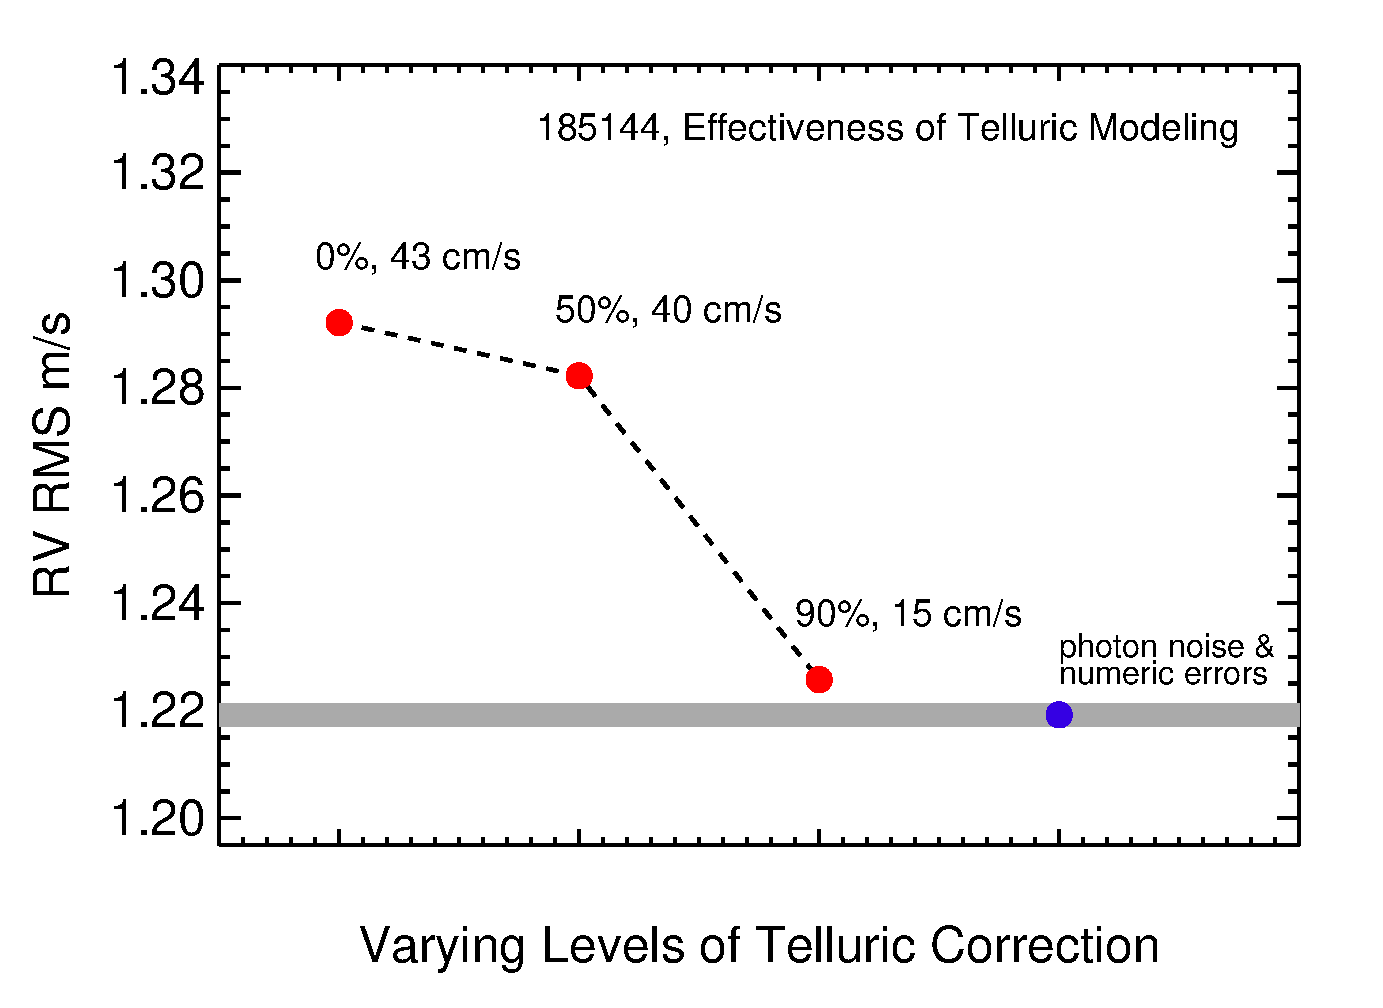
\includegraphics[scale=0.5]{telluric/neid.eps} 
\caption{Improvements in RV RMS for different ``level" of telluric
  modeling/removal. For example, the mid point labeled with ``50\%, 33 cm/s"
  means that if you model your telluric absorption lines to 50\% of
  their original depths, the effects of the residual telluric
  absorption will add 33 cm/s in quadrature to your final RV RMS. The
  blue point marks the RV RMS for simulations with Poisson noise and
  complex IP on HD 185144, which represents the photon-limited RV
  precision (subject to additional numeric or algorithmic errors; see
  Chapter~\ref{chap:conclusion} for more on the limitation of the
  Doppler code).
\label{telluric:fig:neid}}
\end{figure}
%----------------------------------------------------------------

\subsubsection{How about real observations?}

Second, full forward modeling plus some sort of masking for deep
lines. This is the most effective way. Modeling precision of
$\sim$90\% basically bring the adverse effects of tellurics down to
$<$10 cm/s. 90\% is very easy to achieve -- remember the
state-of-the-art is 1-2\%, and even consider errors induced by
modeling residuals caused by atmospheric wind or lack of knowledge on
linelist or broadening parameters or inaccurate knowledge on atmospheric
temperature/pressure profiles. The deep lines may not be modeled very
well. However, the statistical weighting procedure at the very end
will empirically quantify which chunks behave badly due to ineffective
modeling of telluric lines and thus throw out or de-weigh the chunks.

Lead to the next section on deconvolution error.


%%%%%%%%%%%%%%%%%%%%%%%%%%%%%%%%%%%%%%%%%%%%%%%%%%%%%%%%%%%%%%%%%%%%%%%%%%%%
%%%%%%%%%%%%%%%%%%%%%%%%%%%%%%%%%%%%%%%%%%%%%%%%%%%%%%%%%%%%%%%%%%%%%%%%%%%%
\subsection{Discussion and Future Work}\label{keck:telluric:future}

We will try real observation, and see if a priori or floating water
column density parameter works better.

We hope to do a study on M dwarfs, because they are probably worse.

Important for MINERVA, HRS2, HPF2. Crucial for CARMENES, HPF, EPDS, SHREK,
ESPRESSO, SPiRou etc. White paper has suggested improvement on line
lists in HITRAN. EPRV2 has a lot of recommendations. That is the
future direction.
